%width of the three types of plots
\newcommand{\plotwidth}{0.8\linewidth}
\newcommand{\cfinderwidth}{0.96\linewidth}
\newcommand{\otherplotswidth}{0.76\linewidth}

As in the last section, we first discuss our results for the non-overlapping case followed by 
the ones for the overlapping case.

\subsection{Non-overlapping communities}
Figures~\ref{fig:no_iter_no_overlap} and \ref{fig:iter_no_overlap} %and~\ref{fig:compare_iter_no_overlap}
show the plots that we obtained for non-overlapping communities. Figure~\ref{fig:no_iter_no_overlap}
shows tests for the non-iterative method of our algorithm with 5, 10, 15, and 20$\%$ seed nodes per 
community. 

The first observation here is that anything less than 10$\%$ seed nodes per community 
do not give good results. With a seed node percentage of 10$\%$ or more and 
a mixing factor of at most~$0.4$ we achieve an NMI above $0.9$ and can compete with \textit{Infomap}, 
which was deemed to be one the best performing algorithms on the LFR benchmark~\cite{LF09}. 
Above a mixing factor of $0.4$, our algorithm has a worse performance than \textit{Infomap} 
which, curiously enough, achieves an NMI of around 1 till a mixing factor of around 
$0.6$ after which its performance drops steeply. The drop in the performance of our algorithm 
begins earlier but is not as steep. See Figure~\ref{fig:Infomap_etal} for the performance 
of Infomap and other algorithms that were studied in~\cite{LF09}. 

Figure~\ref{fig:iter_no_overlap} shows the results for the iterative approach of 
our algorithm in the non-overlapping case. When compared with the non-iterative approach, 
we found that even after ten iterations there is a significant improvement in 
performance. %(See Figure~\ref{fig:compare_iter_no_overlap}). 
As can be seen, typically with 6$\%$ seed nodes per community we obtain 
acceptable performance (an NMI value of over $0.9$ with the mixing factor 
of up to $0.5$).  


\begin{figure}[h!]
    \centering
    \begin{subfigure}{0.55\textwidth}
    \centering
    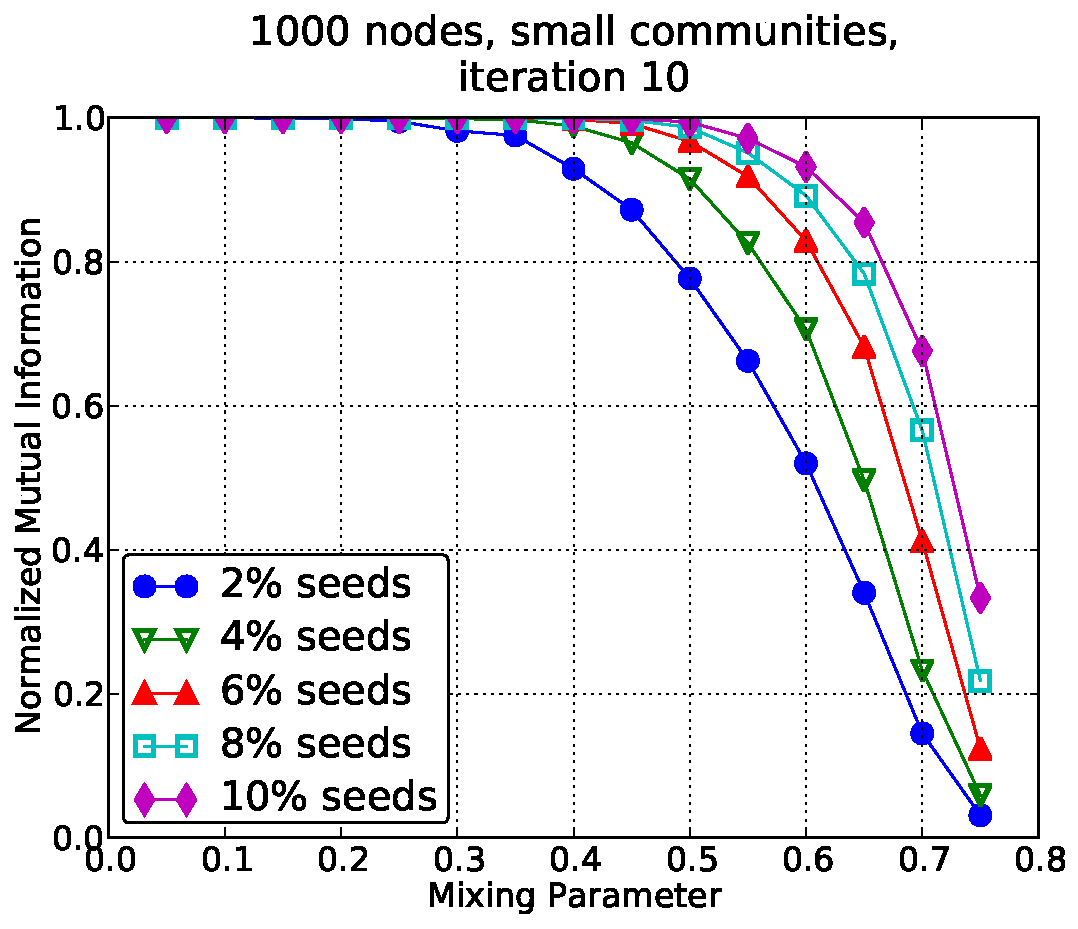
\includegraphics[width=\plotwidth]{plots/nonoverlap_iter_a.pdf}
    \end{subfigure}%
    \begin{subfigure}{0.55\textwidth}
    \centering
    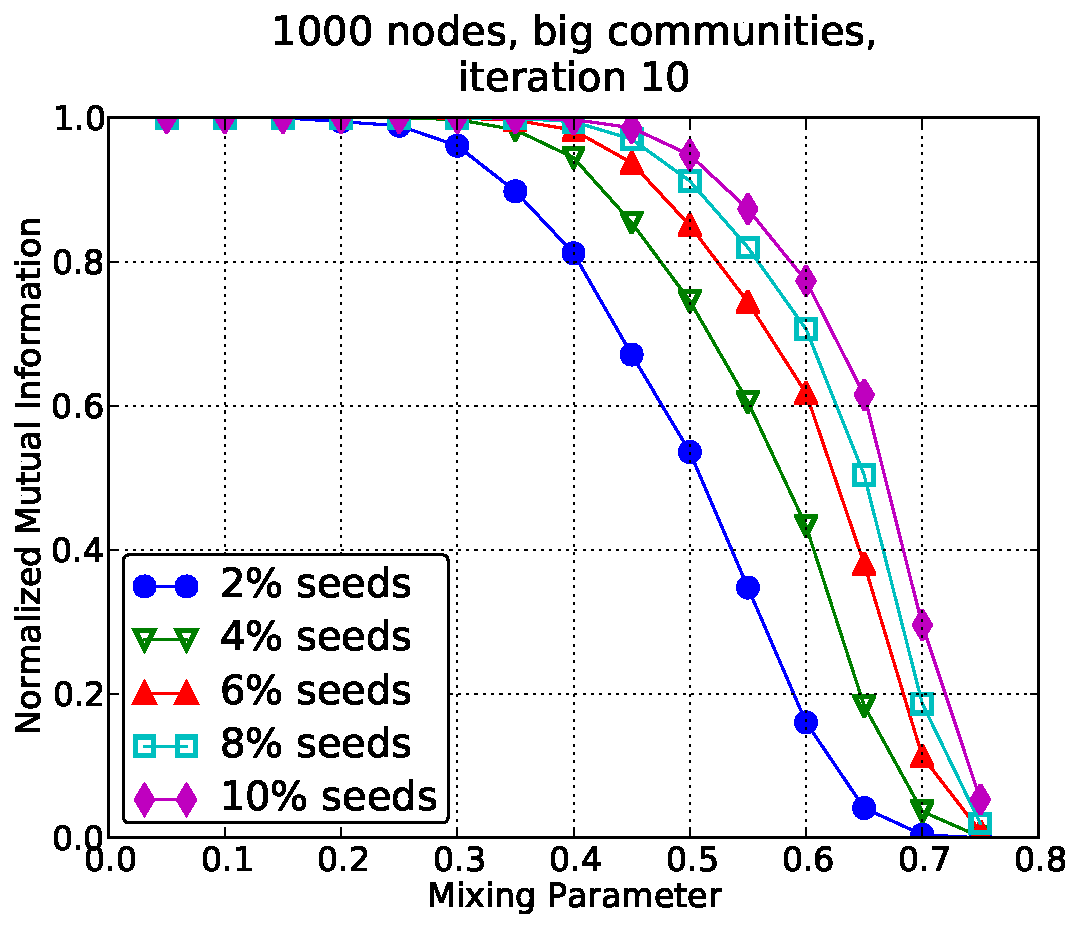
\includegraphics[width=\plotwidth]{plots/nonoverlap_iter_b.pdf}
    \end{subfigure}
    \begin{subfigure}{0.55\textwidth}
    \centering
    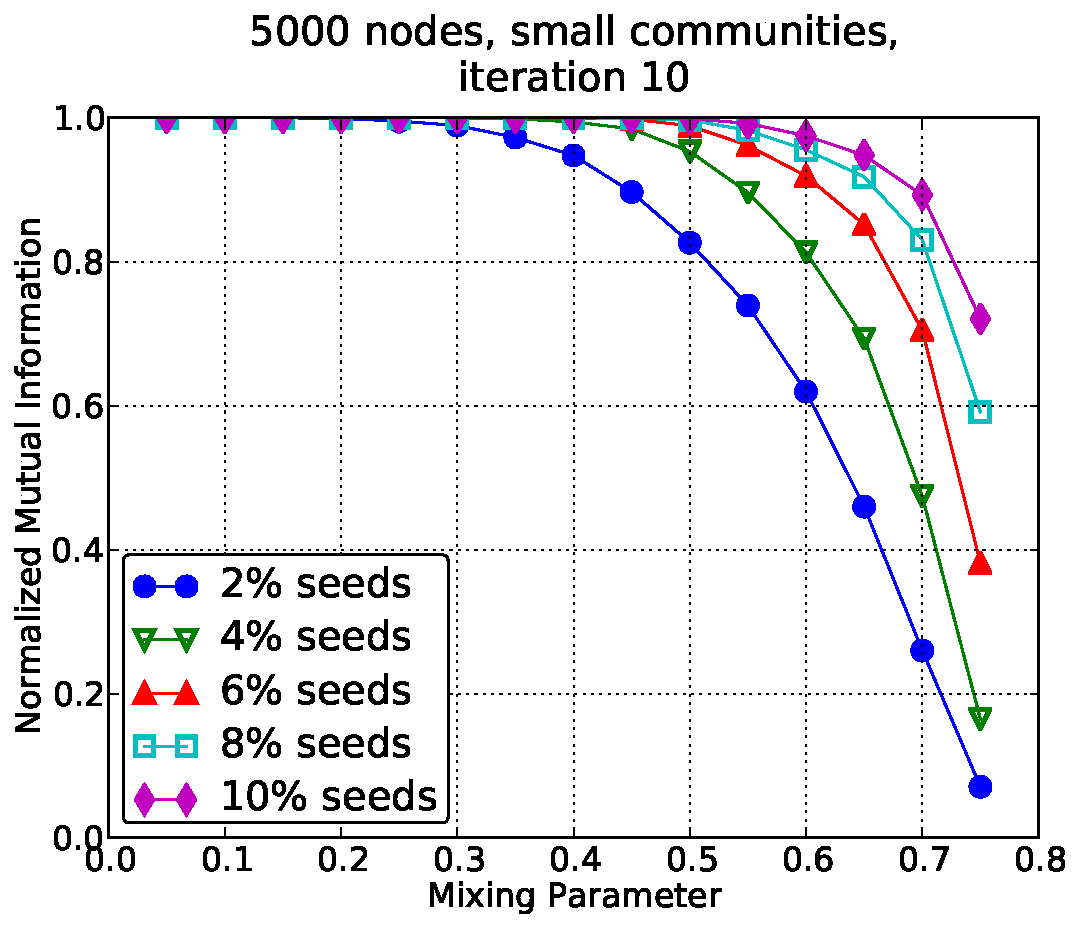
\includegraphics[width=\plotwidth]{plots/nonoverlap_iter_c.pdf}
    \end{subfigure}%
    \begin{subfigure}{0.55\textwidth}
    \centering
    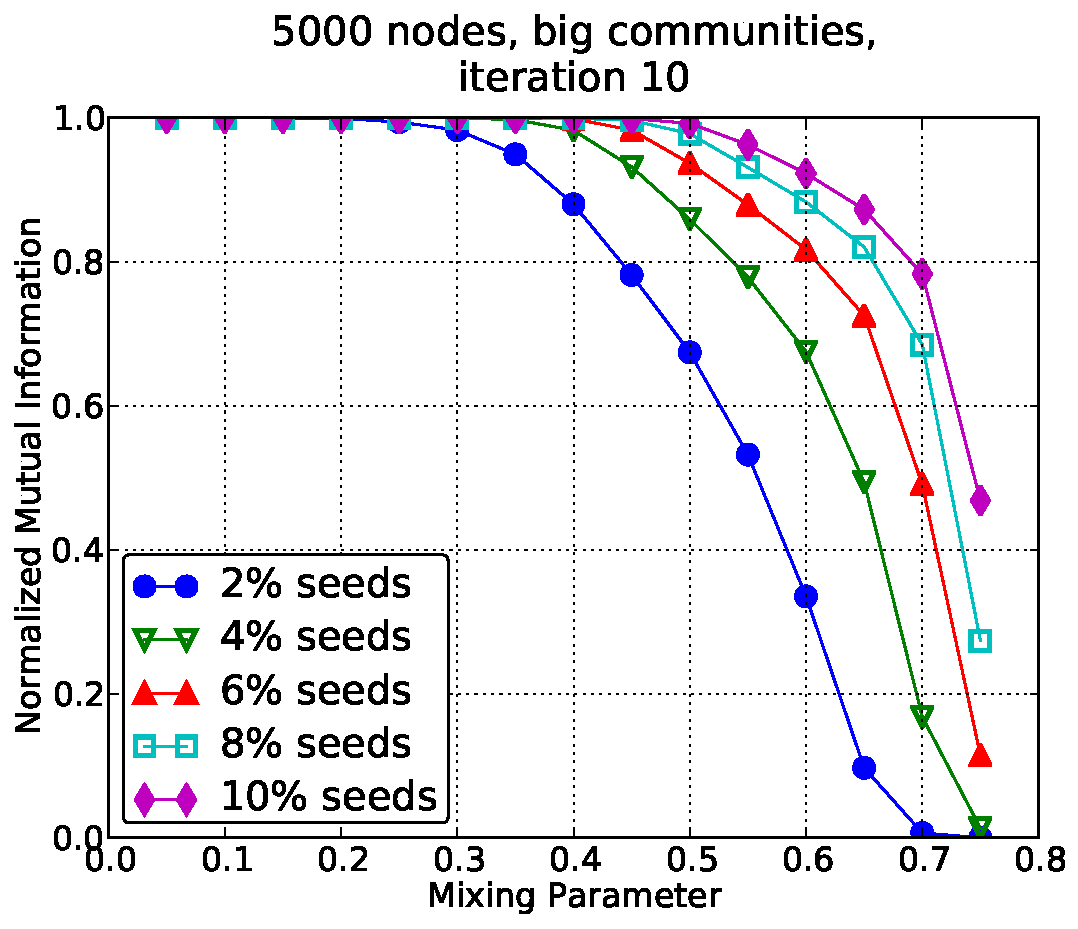
\includegraphics[width=\plotwidth]{plots/nonoverlap_iter_d.pdf}
    \end{subfigure}
    \caption{Iterative method for non-overlapping communities.}\label{fig:iter_no_overlap}
\end{figure}

\begin{figure}[h!]
    \centering
    \begin{subfigure}{0.35\textwidth}
    \centering
    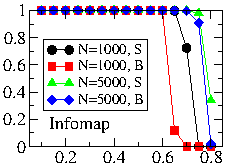
\includegraphics[width=\otherplotswidth]{lfrpaper/1_split_kropped.pdf}
    \end{subfigure}%
    \begin{subfigure}{0.35\textwidth}
    \centering
    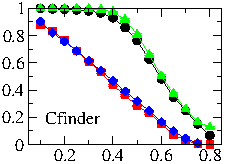
\includegraphics[width=\otherplotswidth]{lfrpaper/2_split_kropped.pdf}
    \end{subfigure}%
    \begin{subfigure}{0.35\textwidth}
    \centering
    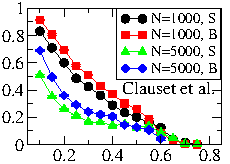
\includegraphics[width=\otherplotswidth]{lfrpaper/3_split_kropped.pdf}
    \end{subfigure}
    \begin{subfigure}{0.35\textwidth}
    \centering
    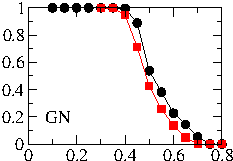
\includegraphics[width=\otherplotswidth]{lfrpaper/4_split_kropped.pdf}
    \end{subfigure}%
    \begin{subfigure}{0.35\textwidth}
    \centering
    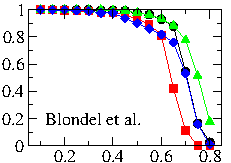
\includegraphics[width=\otherplotswidth]{lfrpaper/5_split_kropped.pdf}
    \end{subfigure}%
    \begin{subfigure}{0.35\textwidth}
    \centering
    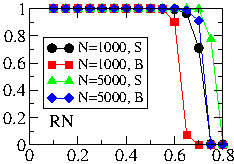
\includegraphics[width=\otherplotswidth]{lfrpaper/6_split_kropped.pdf}
    \end{subfigure}%
    \caption{
        Plots for Infomap, CFinder, the algorithm of Clauset \etal, Girvan-Newman (GN), Blondel \etal, 
        and the Pott's model approach by Ronhovde and Nussinov (RN) on the LFR benchmark for non-overlapping 
		communities. As usual, the NMI-value ($y$-axis) is plotted against the mixing factor ($x$-axis).
        Tests were performed on graphs with 1000 and 5000 nodes with big (B) and small (S) communities.
        Reproduced from Lancichinetti and Fortunato~\cite{LF09}.
    }\label{fig:Infomap_etal}
\end{figure}

\begin{figure}[h!]
    \centering
    \begin{subfigure}{0.55\textwidth}
    \centering
    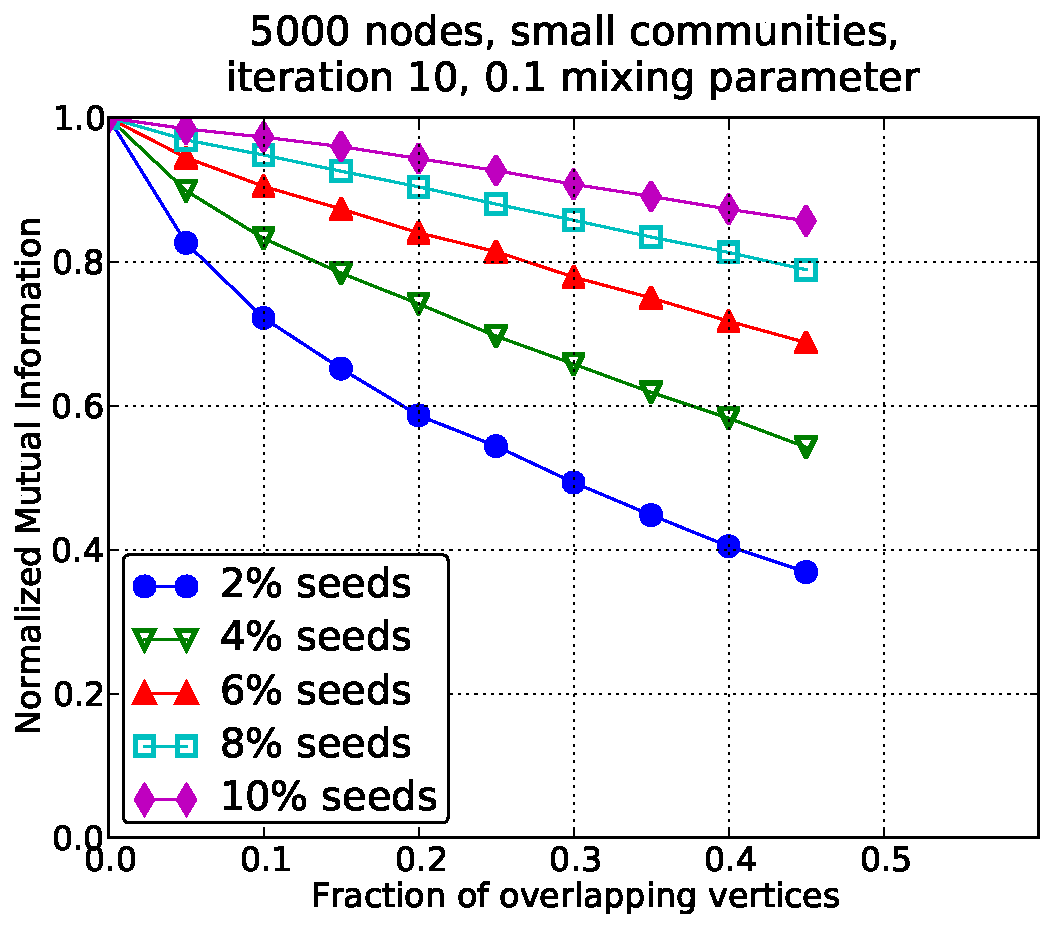
\includegraphics[width=\plotwidth]{plots/overlap_iter_1mu_c.pdf}
    \end{subfigure}%
    \begin{subfigure}{0.55\textwidth}
    \centering
    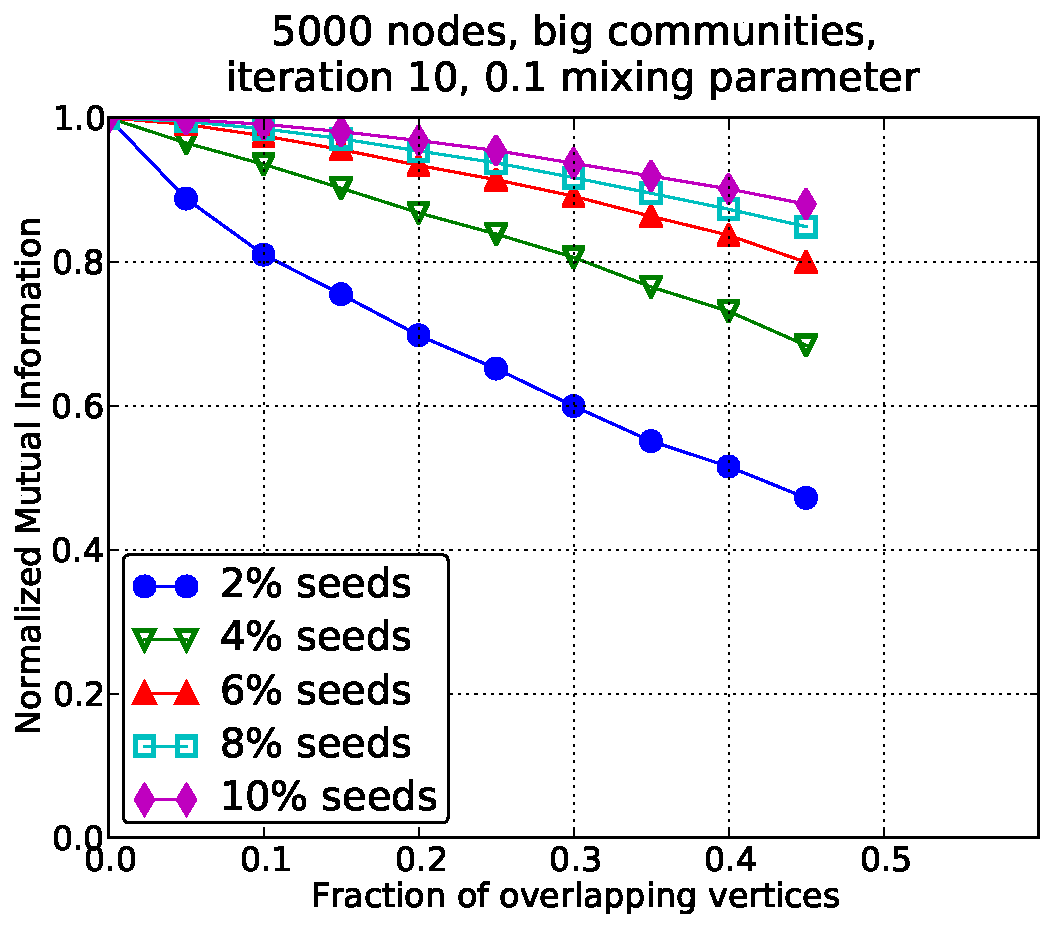
\includegraphics[width=\plotwidth]{plots/overlap_iter_1mu_d.pdf}
    \end{subfigure}
    \begin{subfigure}{0.55\textwidth}
    \centering
    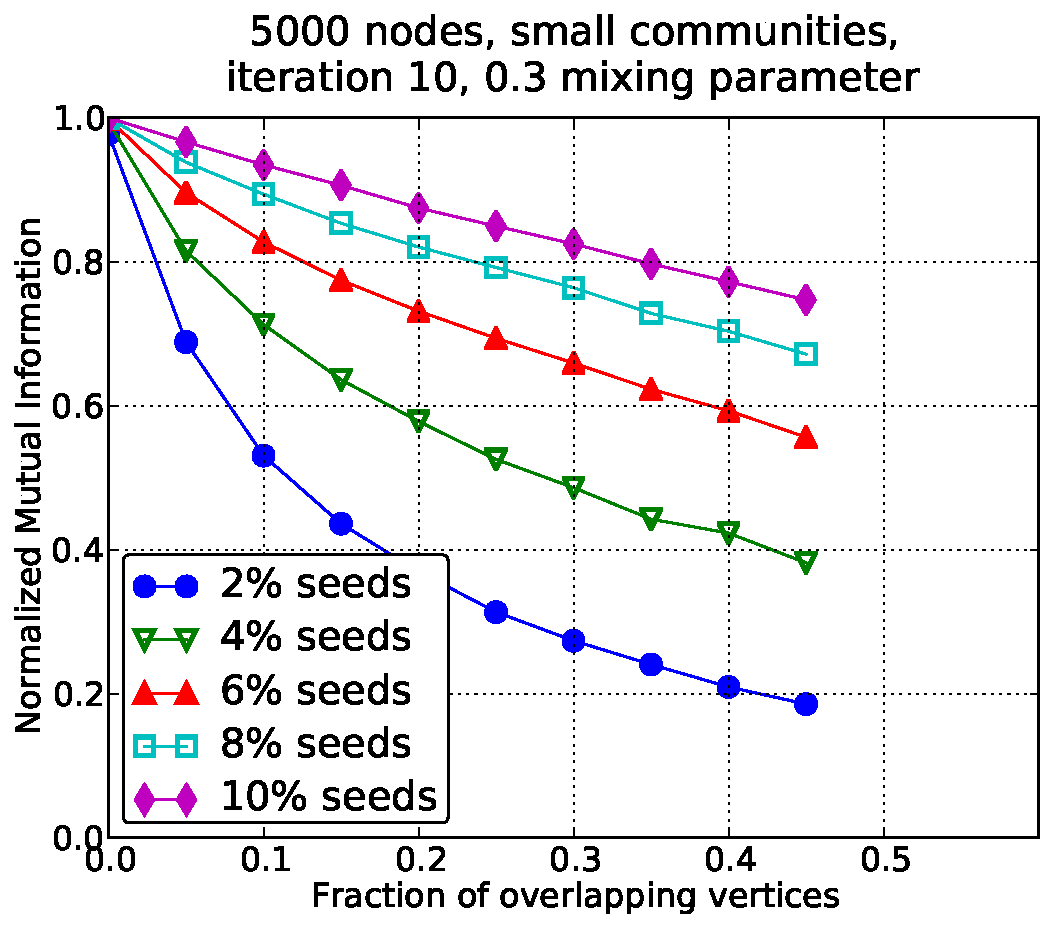
\includegraphics[width=\plotwidth]{plots/overlap_iter_3mu_c.pdf}
    \end{subfigure}%
    \begin{subfigure}{0.55\textwidth}
    \centering
    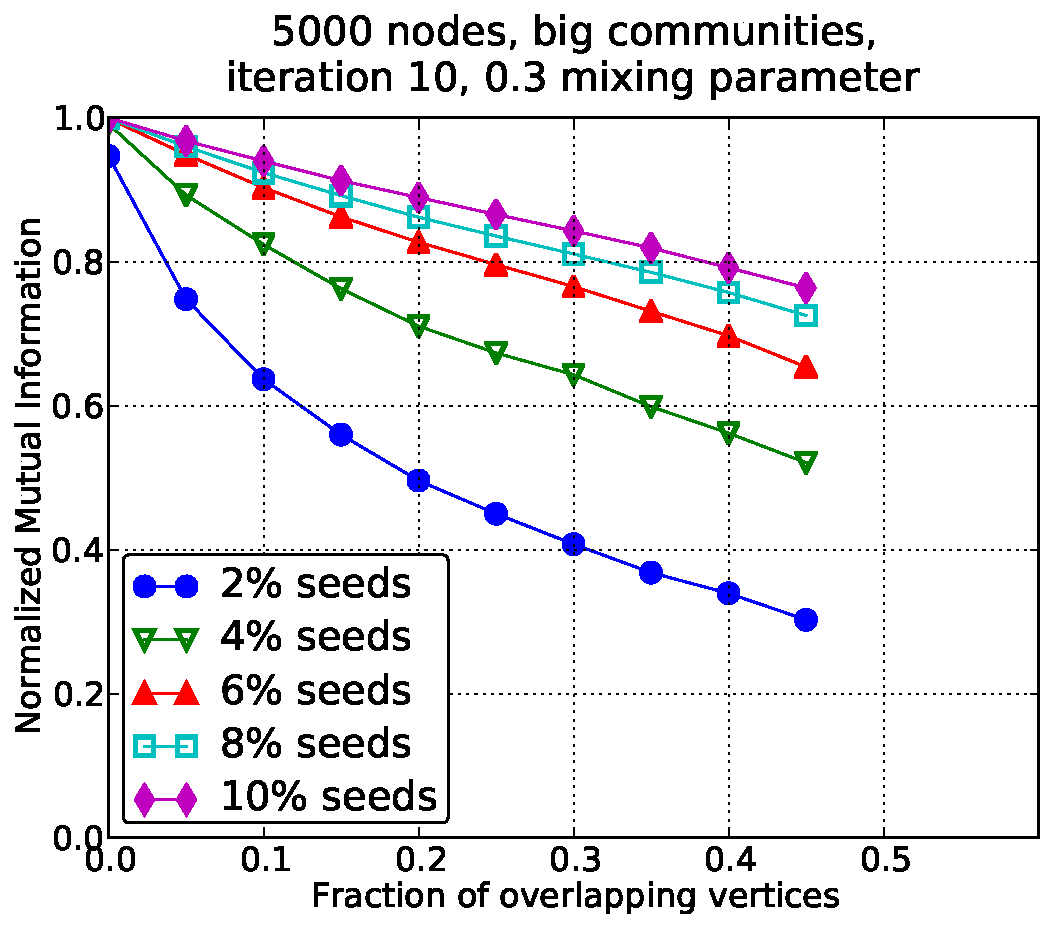
\includegraphics[width=\plotwidth]{plots/overlap_iter_3mu_d.pdf}
    \end{subfigure}
    \caption{Iterative method for overlapping communities on 5000 nodes.}\label{fig:iter_overlap_5000N}
\end{figure}

\begin{figure}[h!]
    \centering
    \begin{subfigure}{0.5\textwidth}
    \centering
    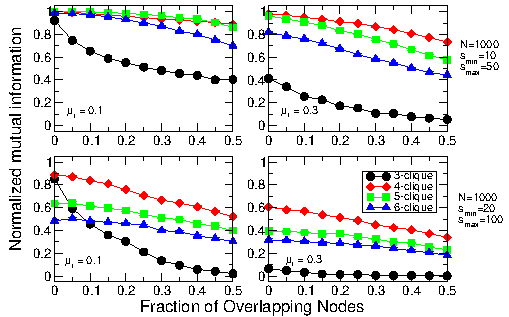
\includegraphics[width=\cfinderwidth]{lfrpaper/fig6.pdf}
    \end{subfigure}%
    \begin{subfigure}{0.5\textwidth}
    \centering
    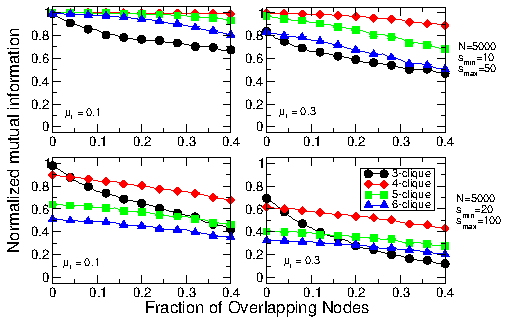
\includegraphics[width=\cfinderwidth]{lfrpaper/fig7.pdf}
    \end{subfigure}%
    \caption{
        Plots for CFinder on the LFR benchmark on graphs with 1000 and 5000 nodes 
		with overlapping communities. Reproduced from Lancichinetti and Fortunato~\cite{LF09}.
    }\label{fig:CFinder_overlapping}
\end{figure}



\subsection{Overlapping communities}
Figures~\ref{fig:no_iter_overlap_1000N} and~\ref{fig:no_iter_overlap_5000N} 
show our results for the overlapping case. In the study of Lancichinetti and Fortunato~\cite{LF09}, 
only one algorithm (\emph{Cfinder}~\cite{PDFV05}) for overlapping communities was benchmarked 
(see Figure~\ref{fig:CFinder_overlapping}). 
The main difference with the non-overlapping case is that typically our algorithm needs a larger 
seed node percentage per community. This is not surprising since in the overlapping case, we would 
need seed nodes from the various overlaps as well as from the non-overlapping portions of communities 
to make a good-enough calculation of the affinities. 

For graphs of both 1000 and 5000 nodes, our algorithm performs better 
than Cfinder up to an overlapping fraction of $0.4$. We stress that Cfinder 
has an exponential worst-case running time and would be infeasible on larger graphs. 
%
Figures~\ref{fig:iter_overlap_1000N} and~\ref{fig:iter_overlap_5000N} show the 
plots for the iterative method (with 10 iterations). 
%A comparison of the non-iterative and iterative method is shown in 
%Figure~\ref{fig:compare_iter_overlap}. 
%Iteration yields an improvement in performance, as measured by the NMI, but it is 
%not as dramatic as in the non-overlapping case with the NMI increase being at most 
%$10\%$ at best. 
The percentage of seed nodes per community required in the 
iterative approach with a mixing factor of $0.3$ is around 8$\%$. 



